% Derived from the parameterized flexible hatch declaration in
% LaTeX-examples-master/tikz/bias-variance/bias-variance.tex.
\documentclass[border=2pt]{standalone}
\usepackage{tikz}
\usetikzlibrary{patterns}
\makeatletter
\tikzset{
  hatch distance/.store in=\hatchdistance,
  hatch distance=10pt,
  hatch thickness/.store in=\hatchthickness,
  hatch thickness=2pt
}
\pgfdeclarepatternformonly[\hatchdistance,\hatchthickness]{flexible hatch}
  {\pgfqpoint{0pt}{0pt}}
  {\pgfqpoint{\hatchdistance}{\hatchdistance}}
  {\pgfpoint{\hatchdistance-1pt}{\hatchdistance-1pt}}
  {
    \pgfsetcolor{\tikz@pattern@color}
    \pgfsetlinewidth{\hatchthickness}
    \pgfpathmoveto{\pgfqpoint{0pt}{0pt}}
    \pgfpathlineto{\pgfqpoint{\hatchdistance}{\hatchdistance}}
    \pgfusepath{stroke}
  }

\begin{document}
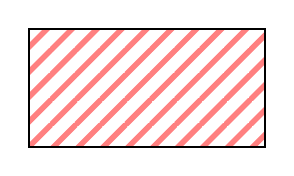
\begin{tikzpicture}
  \fill[pattern=flexible hatch,pattern color=red!50] (0,0) rectangle (3,1.5);
  \draw[thick] (0,0) rectangle (3,1.5);
\end{tikzpicture}
\end{document}
